\section{More details about the Resolved Top Tagger (13 TeV)}
\label{app:TopTagger13TeVMore}
In this Appendix we compare the inputs of the resolved top tagger in 13 TeV data and simulations. The level of agreement of the jet quark-quark gluon likelihood (Fig. \ref{fig:qgid1213TeV}) is insufficient. We are investigating the reasons behind that. Other than that, we notice an overall fair agreement between data and simulations for all the top tagger input variables.

\begin{figure}[htbp]
	\centering
	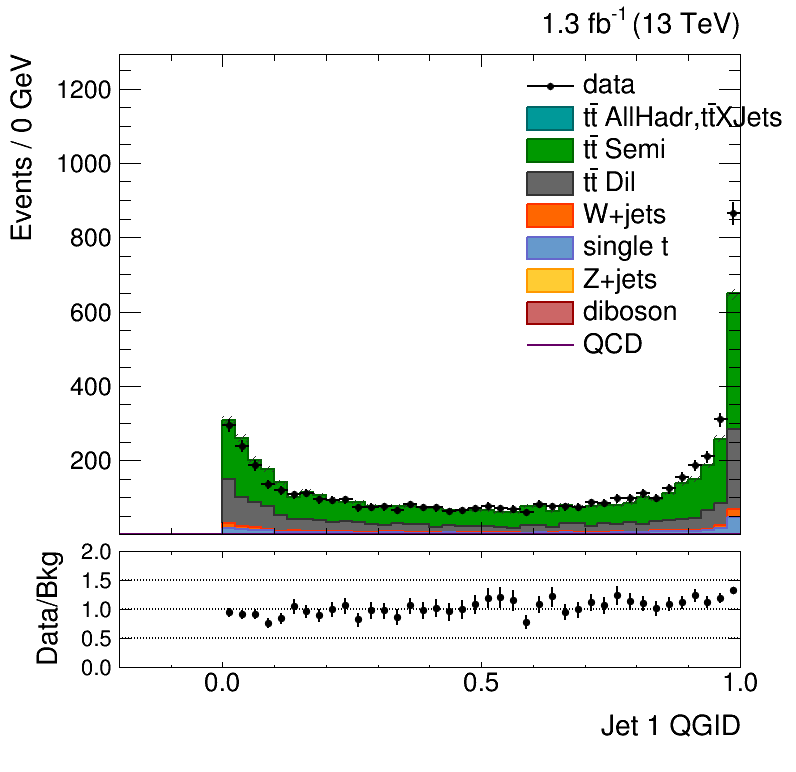
\includegraphics[width=0.48\textwidth]{figures/semilep_1tightmuo_resolved_3ormorejets_2ormorejetWPm_pfmetmore100_pfmtmore40_trigrequestonMC_qgsmearedwith8TeVrecipe_Oct302015/res_hJet1qgid.png}
	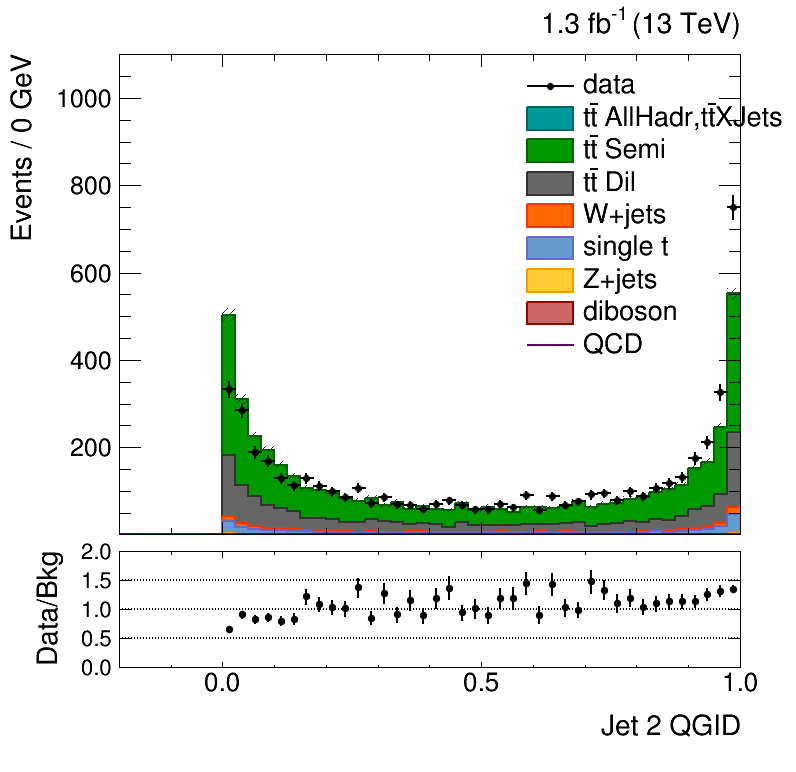
\includegraphics[width=0.48\textwidth]{figures/semilep_1tightmuo_resolved_3ormorejets_2ormorejetWPm_pfmetmore100_pfmtmore40_trigrequestonMC_qgsmearedwith8TeVrecipe_Oct302015/res_hJet2qgid.png}
	\caption{Quark/gluon discriminant output in data and MC of the two jets in the triplet which maximizes the resolved tagger. The jet with the highest-CSV has not been considered.}
	\label{fig:qgid1213TeV}
\end{figure}

\begin{figure}[htbp]
	\centering
	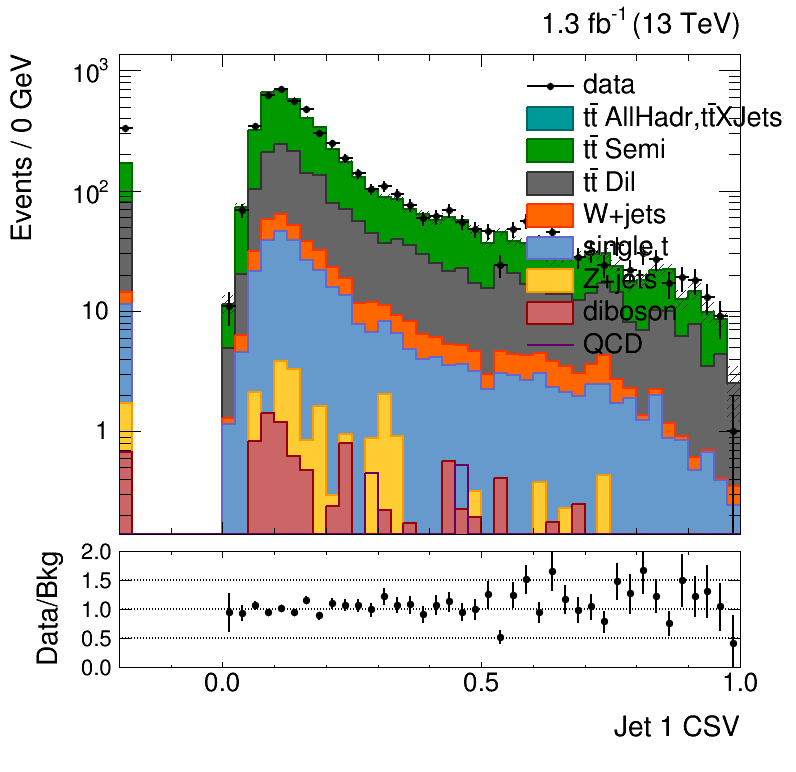
\includegraphics[width=0.48\textwidth]{figures/semilep_1tightmuo_resolved_3ormorejets_2ormorejetWPm_pfmetmore100_pfmtmore40_trigrequestonMC_qgsmearedwith8TeVrecipe_Oct302015/res_hJet1csv.png}
	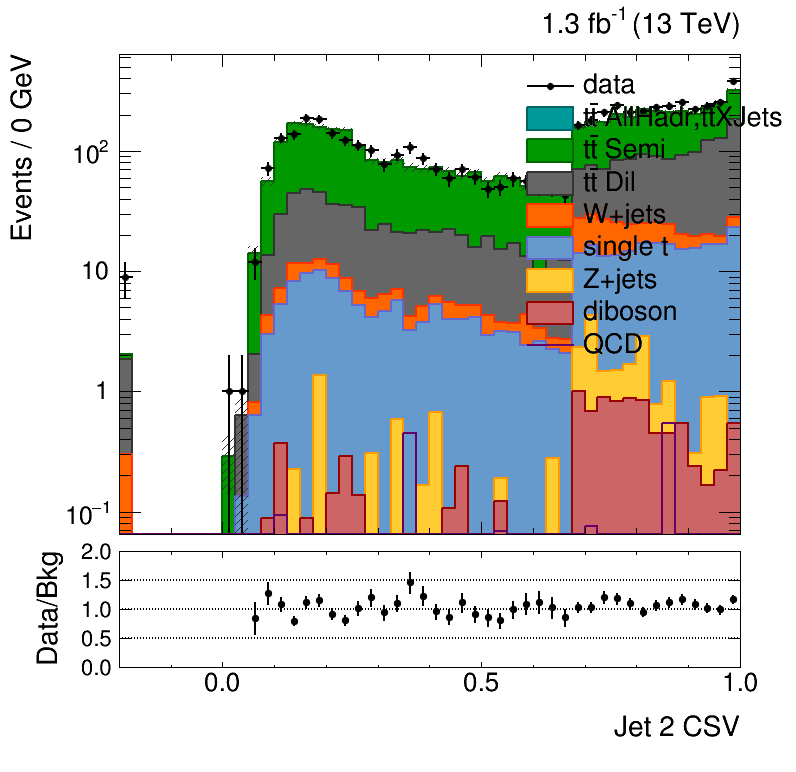
\includegraphics[width=0.48\textwidth]{figures/semilep_1tightmuo_resolved_3ormorejets_2ormorejetWPm_pfmetmore100_pfmtmore40_trigrequestonMC_qgsmearedwith8TeVrecipe_Oct302015/res_hJet2csv.png}
	\caption{CSV output in data and MC of the two jets in the triplet which maximizes the resolved tagger. The jet with the highest-CSV has not been considered.}
	\label{fig:jet12csv}
\end{figure}

\begin{figure}[htbp]
	\centering
	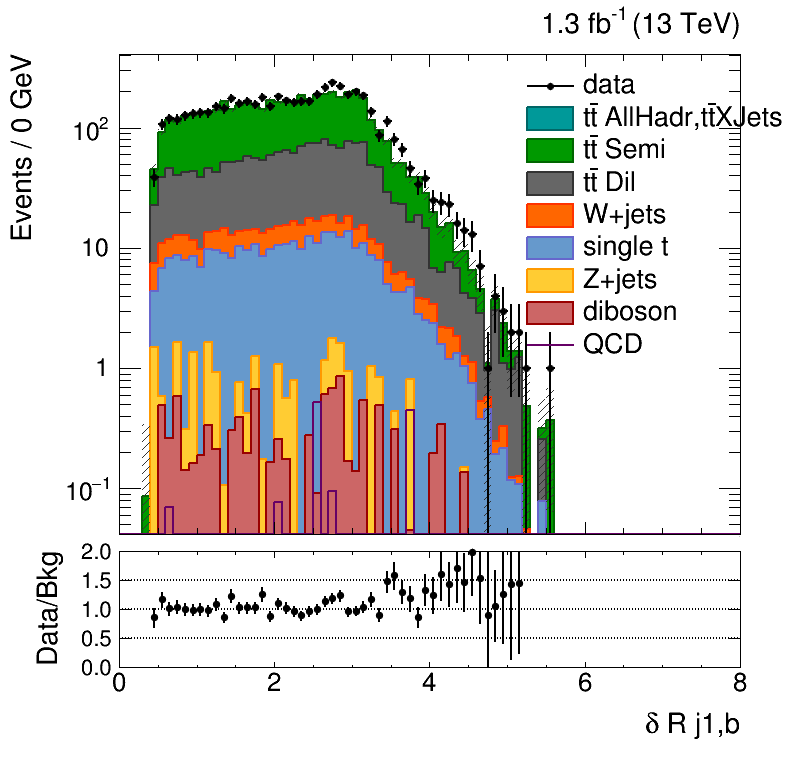
\includegraphics[width=0.48\textwidth]{figures/semilep_1tightmuo_resolved_3ormorejets_2ormorejetWPm_pfmetmore100_pfmtmore40_trigrequestonMC_qgsmearedwith8TeVrecipe_Oct302015/hResBDTDRj1b.png}
	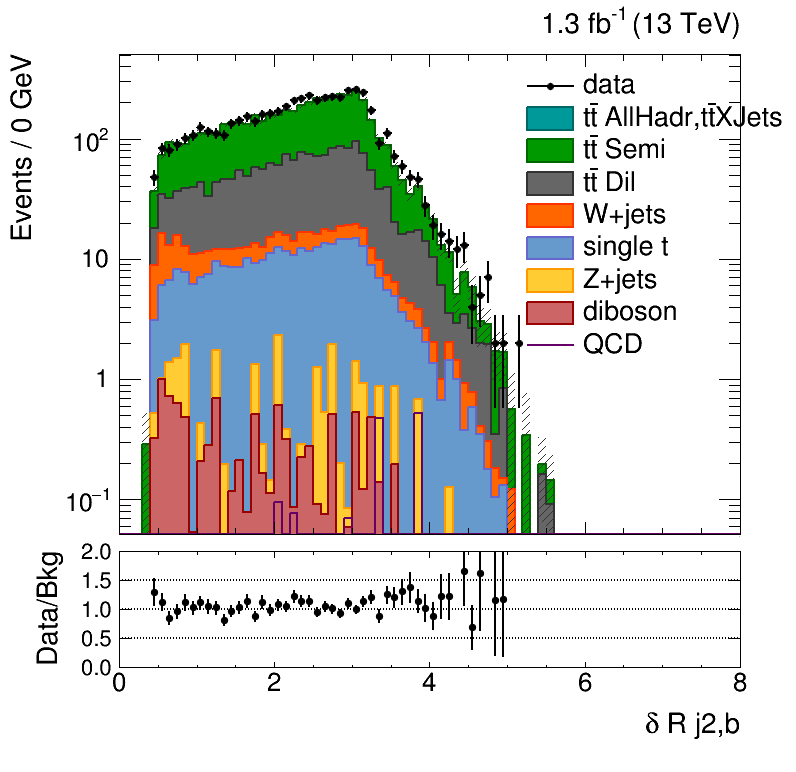
\includegraphics[width=0.48\textwidth]{figures/semilep_1tightmuo_resolved_3ormorejets_2ormorejetWPm_pfmetmore100_pfmtmore40_trigrequestonMC_qgsmearedwith8TeVrecipe_Oct302015/hResBDTDRj2b.png}
	\caption{Data and MC comparisons for the $\Delta$ R between the first and the third jet (left), the second and the third jet (right) of the triplet which maximizes the resolved tagger. The jets have been ordered in decreasing CSV output.}
	\label{fig:dRj12b13TeV}
\end{figure}

\begin{figure}[htbp]
	\centering
	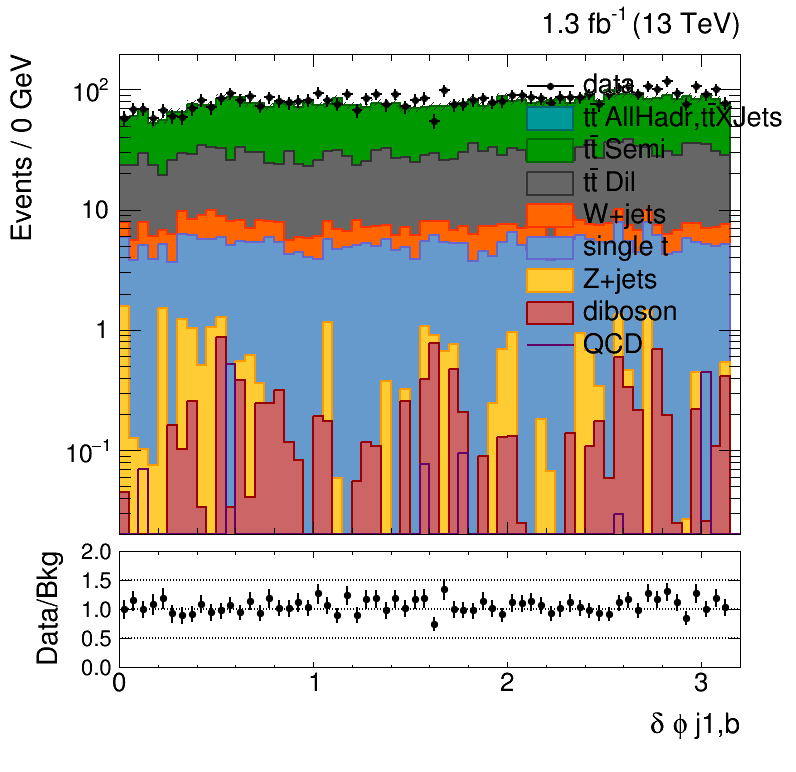
\includegraphics[width=0.48\textwidth]{figures/semilep_1tightmuo_resolved_3ormorejets_2ormorejetWPm_pfmetmore100_pfmtmore40_trigrequestonMC_qgsmearedwith8TeVrecipe_Oct302015/hResBDTDPhij1b.png}
	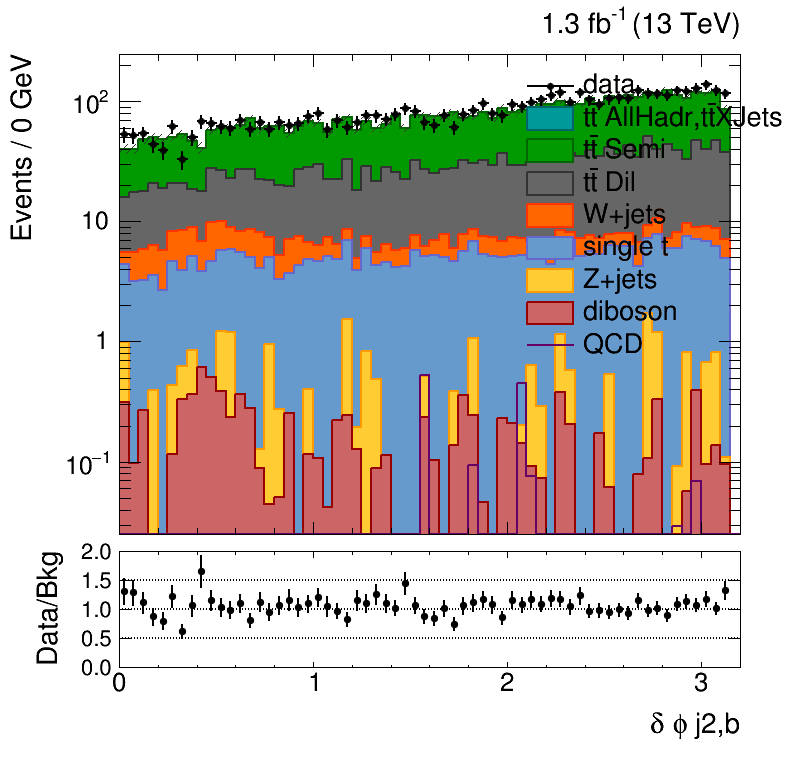
\includegraphics[width=0.48\textwidth]{figures/semilep_1tightmuo_resolved_3ormorejets_2ormorejetWPm_pfmetmore100_pfmtmore40_trigrequestonMC_qgsmearedwith8TeVrecipe_Oct302015/hResBDTDPhij2b.png}
	\caption{Data and MC comparisons for the $\Delta \phi$  between the first and the third jet (left), the second and the third jet (right) of the triplet which maximizes the resolved tagger. The jets have been ordered in decreasing CSV output.}
	\label{fig:dphij12b13TeV}
\end{figure}

\begin{figure}[htbp]
	\centering
	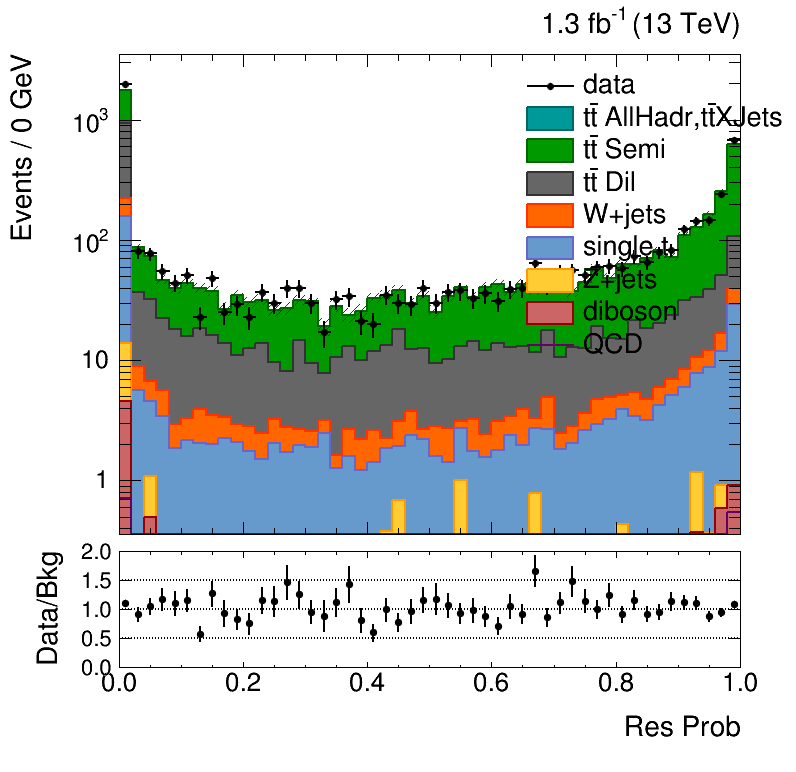
\includegraphics[width=0.48\textwidth]{figures/semilep_1tightmuo_resolved_3ormorejets_2ormorejetWPm_pfmetmore100_pfmtmore40_trigrequestonMC_qgsmearedwith8TeVrecipe_Oct302015/hResProb.png}
	\caption{Fit probability in Data and MC. The fit probability variable has been described in Sec. \ref{subsec:sel_toptag_resolved}.}
	\label{fig:fitprob13TeV}
\end{figure}